% Autor: Leonhard Segger, Alexander Neuwirth
% Datum: 2017-10-30
\documentclass[
	% Papierformat
	a4paper,
	% Schriftgröße (beliebige Größen mit „fontsize=Xpt“)
	12pt,
	% Schreibt die Papiergröße korrekt ins Ausgabedokument
	pagesize,
	% Sprache für z.B. Babel
	ngerman
]{scrartcl}

% Achtung: Die Reihenfolge der Pakete kann (leider) wichtig sein!
% Insbesondere sollten (so wie hier) babel, fontenc und inputenc (in dieser
% Reihenfolge) als Erstes und hyperref und cleveref (Reihenfolge auch hier
% beachten) als Letztes geladen werden!

\usepackage{tikz}
\usetikzlibrary{calc,patterns,angles,quotes} % loads some tikz extensions\usepackage{tikz}
\usetikzlibrary{babel}

% Silbentrennung etc.; Sprache wird durch Option bei \documentclass festgelegt
\usepackage{babel}
% Verwendung der Zeichentabelle T1 (Sonderzeichen etc.)
\usepackage[T1]{fontenc}
% Legt die Zeichenkodierung der Eingabedatei fest, z.B. UTF-8
\usepackage[utf8]{inputenc}
% Schriftart
\usepackage{lmodern}
% Zusätzliche Sonderzeichen
\usepackage{textcomp}

% Mathepaket (intlimits: Grenzen über/unter Integralzeichen)
\usepackage[intlimits]{amsmath}
% Ermöglicht die Nutzung von \SI{Zahl}{Einheit} u.a.
\usepackage{siunitx}
% Zum flexiblen Einbinden von Grafiken (\includegraphics)
\usepackage{graphicx}
% Abbildungen im Fließtext
\usepackage{wrapfig}
% Abbildungen nebeneinander (subfigure, subtable)
\usepackage{subcaption}
% Funktionen für Anführungszeichen
\usepackage{csquotes}
\MakeOuterQuote{"}
% Zitieren, Bibliographie
\usepackage{biblatex}


% Zur Darstellung von Webadressen
\usepackage{url}
%chemische Formeln
\usepackage[version=4]{mhchem}
% siunitx: Deutsche Ausgabe, Messfehler getrennt mit ± ausgeben
\usepackage{floatrow}
\floatsetup[table]{capposition=top}
\usepackage{float}
% Verlinkt Textstellen im PDF-Dokument
\usepackage[unicode]{hyperref}
% "Schlaue" Referenzen (nach hyperref laden!)
\usepackage{cleveref}
\sisetup{
	locale=DE,
	separate-uncertainty
}
\bibliography{14Mo_O6_09-07-2018_References}

\begin{document}
	
	\begin{titlepage}
		\centering
		{\scshape\LARGE Versuchsbericht zu \par}
		\vspace{1cm}
		{\scshape\huge O6 - Optische Abbildungen und digitale Kamera \par}
		\vspace{2.5cm}
		{\LARGE Gruppe 14Mo \par}
		\vspace{0.5cm}
		
		{\large Alexander Neuwirth (E-Mail: a\_neuw01@wwu.de) \par}
		{\large Leonhard Segger (E-Mail: l\_segg03@uni-muenster.de) \par}
		\vfill
		
		durchgeführt am 09.07.2018\par
		betreut von\par
		{\large Robert Schneider} 
		
		\vfill
		
		{\large \today\par}
	\end{titlepage}
	\tableofcontents
	\newpage

	%TODO mehr TODO in Default	

	\section{Kurzfassung}
	%TODO Hypothese	und deren Ergebnis, wenn Hypothese ist, dass nur Theorie erfüllt, sagen: Erwartung: Theorie aus einführung (mit reflink) erfüllt
	%TODO Ergebnisse, auch Zahlen, mindestens wenn's halbwegs Sinn ergibt
	%TODO Was wurde gemacht
	%TODO manche leute wollen Passiv oder "man", manche nicht
	Es wird das Auflösungsvermögen und die Schärfentiefe einer Digitalkamera mit unterschiedlichen Optiken vor dem Sensor untersucht.
	%TODO Tiefenschärfe abgeschätzt vs Fourier oder so in Abhängigkeit von Blende
	%TODO Einzellinse: Auflösung in Abhängikeit von Blendendurchmesser mit Siemens + MTF-Kurve (Tipp unten)
	%TODO Lochblende: Auflösung + anhand der notwendigen Belichtungszeit die Blendenöffnung der Lochblende abschötzen
	\section{Methoden}
	%einer will Präsens
	Für die Versuchsdurchführung wird eine Nikon D3200 verwendet, die zunächst auf die Werkseinstellungen zurückgesetzt wird. %sellout
	Als erstes wird ein Nikkor 50 mm Objektiv an die Kamera angebracht und die Kamera auf den rechten, um \SI{45}{\degree} gekippten Teil des in \cref{fig_testchart} dargestellten Testcharts ausgerichtet.
	Mithilfe von digitalen Zoom wird die Mitte der Skala von \SIrange{-10}{10}{\centi \meter} am Objektiv scharf gestellt.
	Dann werden für alle acht Blendenzahlen in ganzen Stufen von 1 bis 22 je ein Bild des Testcharts aufgenommen, um die Schärfentiefe in Abhängigkeit von der Blendenzahl bestimmen zu können.
	Die Belichtungszeit wählt die Kamera automatisch.
	
	Das Objektiv wird durch eine Einzellinse mit einer Brennweite von \SI{60}{\milli \meter} ersetzt.
	Um die 	Auflösung bestimmen zu können, wird für drei verschiedene Durchmesser der eingeschraubter Blende und ohne zusätzliche Blende je eine Fotografie von zwei Siemenssternen angefertigt.
	Einer der Siemenssterne befindet sich dabei möglichst nah an der Mitte und einer am Rand der Fotografie.
	Die Belichtungszeit wird dabei bei Halbierung des Blendendurchmessers vervierfacht, um die Belichtung der Bilder konstant zu halten. %TODO vlt. erklären, da eigentlich sschwarz/weiß-werte vergleichen gewollt.
	Das Scharfstellen erfolgt durch Drehen des Tubus der Einzellinse.
	
	Zuletzt werden Linse und Blende durch eine Lochblende mit einem deutlich kleineren Durchmesser ersetzt. %TODO maybe für Hypothese bahaupten mit Auge abgeschätzt E-7m
	Die Kamera wird deutlich näher am Testchart positioniert.
	
	Bei allen Fotografien wird der Abstand der Kamera vom Testchart mit einem Maßband gemessen und notiert.
	%TODO Imagej für Auswertung erwähnen`? vmtl nicht.
	%TODO bissl erwähnen, wie ausgewertet wird, wenn nicht unten klar.
	\begin{figure}[H] 
		\includegraphics[width=1\textwidth]{fig_Testchart}
		\centering
		\caption{Das Testchart, das verwendet wurde, um die Eigenschaften der Kamera und Optiken zu untersuchen. Entnommen aus \cite{Testchart}} %TODO Optiken gutes Wort?
		\label{fig_testchart}
		\centering
	\end{figure}
	%Tipp: Mit der beschriebenen Methode liefert der Siemensstern nicht die Frequenz, für die MTF=0,5 gilt. Wie groß ist die MTF der ermittelten Frequenz?
	\section{Ergebnisse und Diskussion}
	%TODO Unsicherheiten
	

	\subsection{Beobachtung und Datenanalyse}
	%TODO Einflüsse von veränderten Parametern auf Messung
	\subsubsection{Unsicherheiten} %TODO GGF IN DATENANYLSY
Die Unsicherheiten werden gemäß GUM ermittelt. 
	Außerdem wird für Unsicherheitsrechnungen die Python-Bibliothek "uncertainties" verwendet.
	\begin{description}
		\item[Abstandmessung:] Die Messung des Abstands zwischen Kamera und Testchart wurde mit einem Maßband durchgeführt. 
			Dabei wurde die Unsicherheit mit \SI{0,81}{cm} abgeschätzt (dreieckige WDF).
		\item[Pixelanzahl:] Die farblichen Übergänge der Pixel waren nicht eindeutig von schwarz zu weiß. 
			Deshalb wurde hierbei eine Unsicherheit von \SI{3}{px} verwendet.  %TODO hast du was ähnliches gemacht oder net...
		\item[Subjektive Schärfe:] Inwiefern die Angabe eines Fehlers für die angabe eines subjektiven Werts sinnvoll ist, ist fraglich. Dennoch soll hier mit einer Unsicherheit von \SI{1}{cm} auf der schrägen Skala angenommen werden, um sicherzugehen, dass immer möglichst gleich scharfe Bereiche gewählt werden.  %TODO lul
	\end{description}

	\subsubsection{Untersuchung der Schärfentiefe}
	\subsubsection*{Theoretische Berechnung}
	Die Schärfentiefe $S_\text{theo}$ ergibts sich aus der Entfernung zwischen Nah- und Fernpunkt.
	Also $S_\text{theo}= |d_h - d_f|$.
	Mit den in der Einführung gegebenen Formeln: %TODO cref
	\begin{equation}
		d_n = \frac{g\cdot (d_h-f)}{(d_h-f)+(g-f)}
	\end{equation}
	\begin{equation}
		d_f = 
		\begin{cases}
			\frac{g\cdot (d_h - f)}{(d_h-f)+(f-g)} & \text{wenn }  g < d_h \\
			\infty & \text{wenn }  g \geq d_h \\
		\end{cases}
	\end{equation}
	wobei $d_h$ die hyperfokale Entfernung ist:
	\begin{equation}
		d_h = \frac{f^2}{k\cdot Z} + f
	\end{equation}
	Es folgt also eine Schärfentiefe von:
	\begin{equation}
		S_\text{theo} = \left| \frac{2f^2 g k Z (f-g)}{f^4-k^2 Z^2 (f-g)^2} \right|
		\label{eq_scharf_tief}
	\end{equation}
	Dabei ist $Z$ definiert als $D_B/1500$. 
	$D_B$ ist die Bilddiagonale. 
	Sie wurde berechnet durch die Größe eines Pixels und die Auflösung der Kamera mit 6016 x 4000 Pixeln.
	Eine Strecke von \SI{2}{cm} wurde mit \SI{474+-3} Pixel aufgelöst, das heißt:
	\begin{equation}
		D_B = \frac{\SI{2}{cm}}{\SI{474+-3}{px}}\cdot \sqrt{\SI{6016}{px}^2+\SI{4000}{px}^2} = \SI{30,5+-0,2}{cm}
	\end{equation}
	Die Brennweite des Objektivs $f$ beträgt \SI{50}{mm}.
	Die Messung des Abstands zwischen Testchart und Kamera ergab $g=\SI{64+-0,81}{cm}$
	Einsetzten der jeweiligen $k$ ergibt die Schärfentiefen in \cref{tab_theo_scharf_tief}.

	\begin{table}[H]
		\centering
		\begin{tabular}{ c | c }
			$k$ & $S_\text{theo}$ \\ \hline
			1,8 & \SI{11,1 +- 0,3}{cm} \\
			2,8 & \SI{17,5 +- 0,5}{cm} \\
			4 & \SI{25,5 +- 0,7}{cm} \\
			5,6 & \SI{37,7 +- 1,1}{cm} \\
			8 & \SI{57,6 +- 1,9}{cm} \\
			11 & \SI{93,6 +- 3,6}{cm} \\
			16 & \SI{239,4 +- 16,8}{cm} \\
			22 & \SI{1180,0 +- 318,1}{cm} \\
		\end{tabular}
		\caption{Die nach \cref{eq_scharf_tief} berechneten Schärfentiefen. } %TODO Eq params 
		\label{tab_theo_scharf_tief} 
	\end{table}

	\subsubsection*{Subjektive Schärfentiefe}
	Die schräge Skala ist in einem Winkel von \SI{45+-5}{\degree} gekippt.
	Es ergibt sich ein Faktor $1/\sqrt{2\pm 0,3}$ für die Umrechnung der Skala in Schärfentiefe, welche parallel zur Optischen Achse gemessen wird.
	In \cref{tab_subj_scharf_tief} sind die subjektiven Schärfentiefen in Abhängikeit von $k$ aufgelistet.

	\begin{table}[H]
		\centering
		\begin{tabular}{ c | c }
			$k$ & $S_\text{subj}$ \\ \hline
			1,8 & \SI{4,2 +- 0,8}{cm} \\
			2,8 & \SI{6,4 +- 0,9}{cm} \\
			4 & \SI{9,2 +- 1,1}{cm} \\
			5,6 & \SI{16,3 +- 1,6}{cm} \\
			8 & $\geq\SI{20}{cm}$ \\
			11 & $\geq\SI{20}{cm}$ \\
			16 & $\geq\SI{20}{cm}$ \\
			22 & $\geq\SI{20}{cm}$ 
		\end{tabular}
		\caption{Die subjektiven Schärfentiefen.} %TODO Eq params 
		\label{tab_theo_scharf_tief} 
	\end{table}

	\begin{figure}[H]  %TODO ist eig. mehr für Diskussion gedacht
		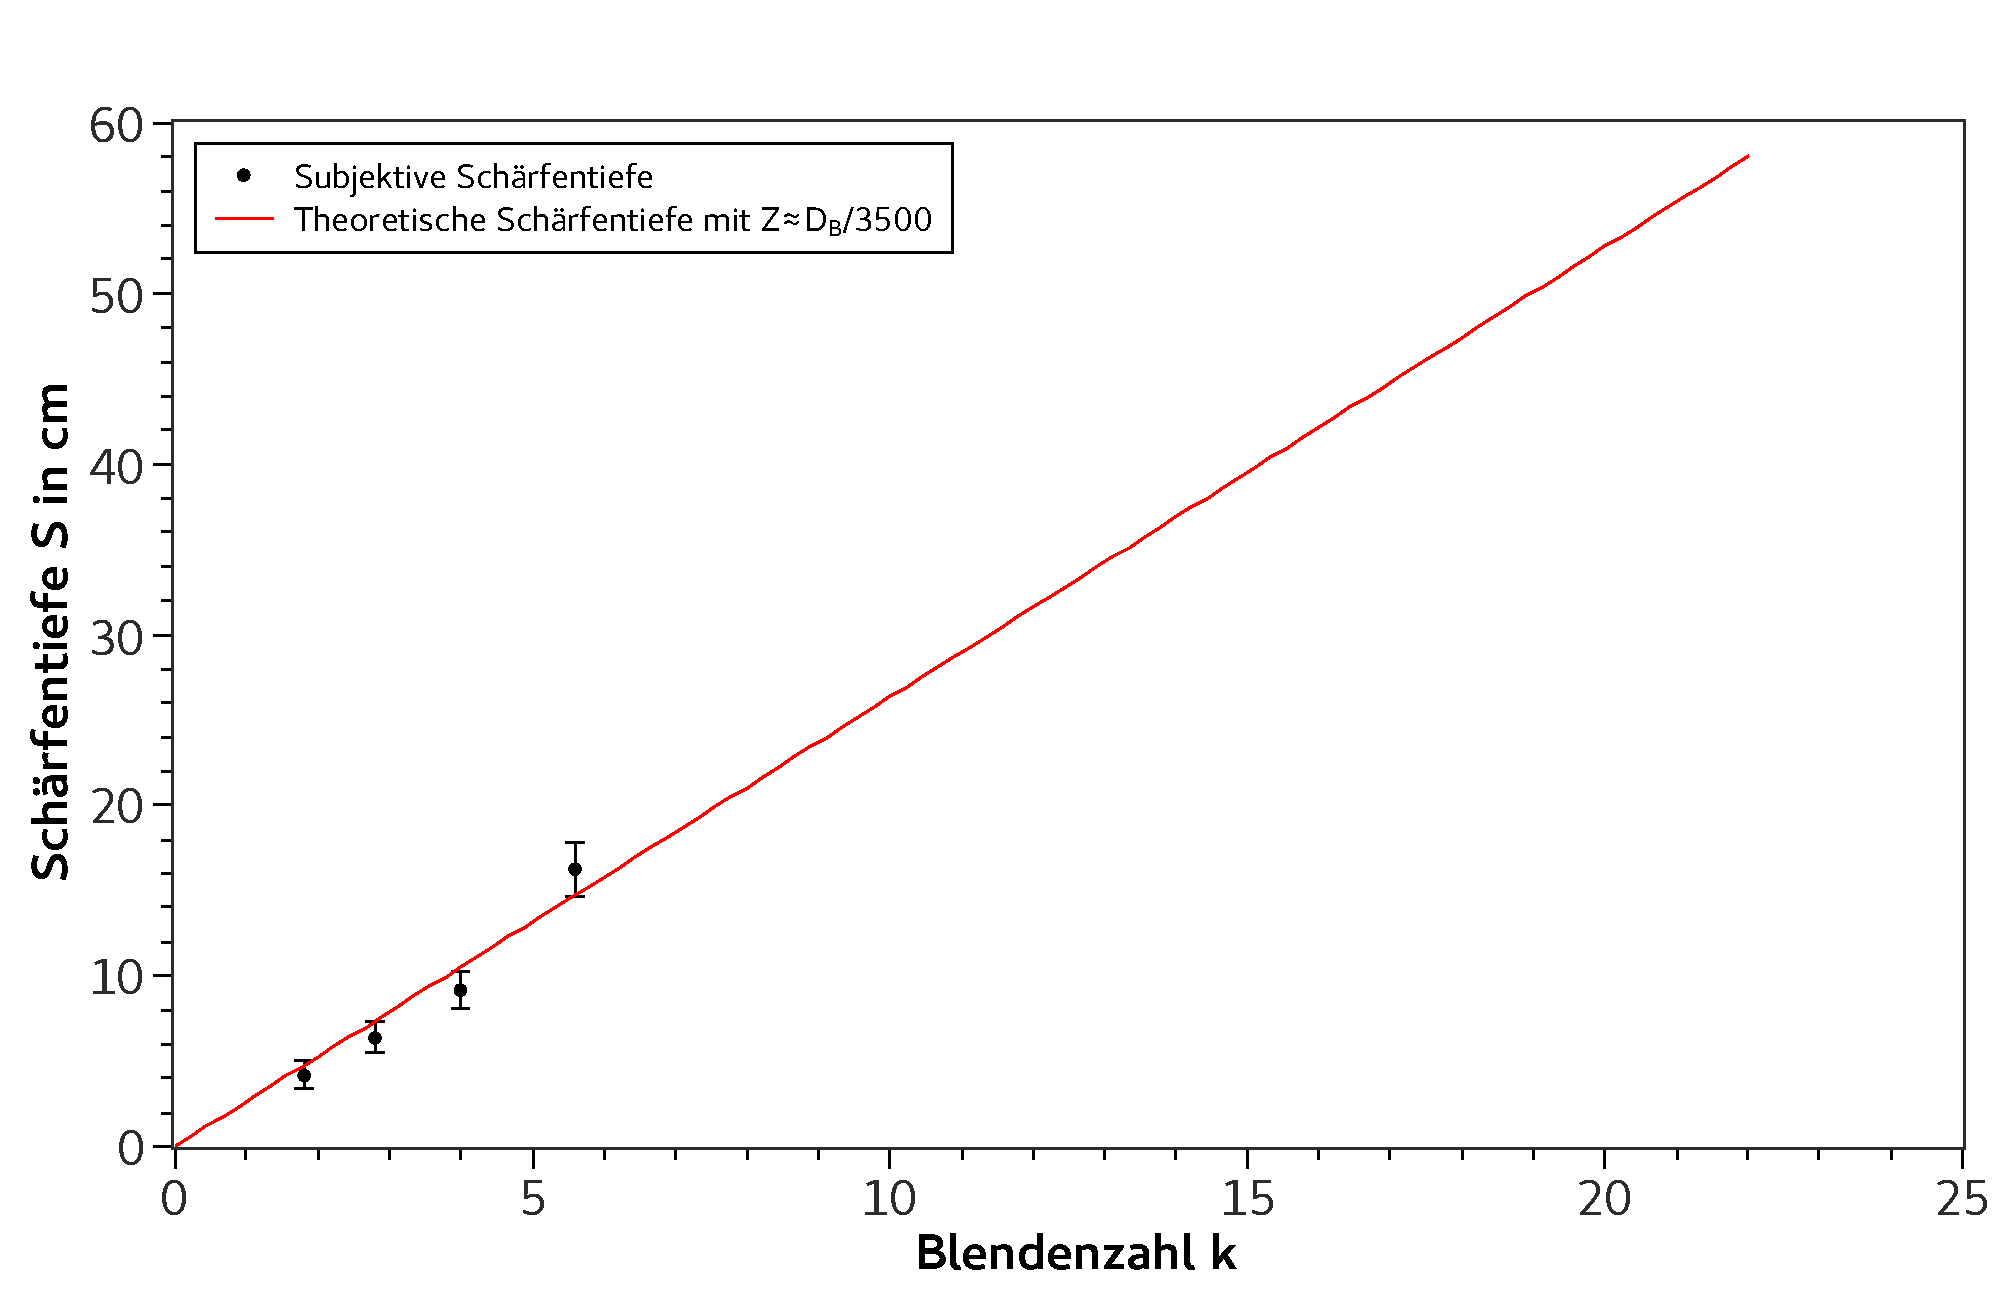
\includegraphics[width=1\textwidth]{fig_scharf_tief}
		\centering
		\caption{Die schwarzen Messpunkte sind die subjektiven Schärfentiefen die noch mit dem Testchart erkennbar waren. 
			Die rote Funktion ist theoretische Schärfentiefe nach \cref{eq_scharf_tief} mit entsprechenden Parametern.
			Die einzige Änderung die durchgeführt wurde ist die Skalierung der Durchmessergrenze $Z$ der Zerstreuungskreise mit einem Faktor von ca. 3/7.}
		\label{fig_scharf_tief}
		\centering
	\end{figure}
	
	%TODO divergiert nahe 20 weil d_h ~ g => erklärt hohe theo schärfentiefe
	\begin{figure}[H]  %TODO ist eig. mehr für Diskussion gedacht
		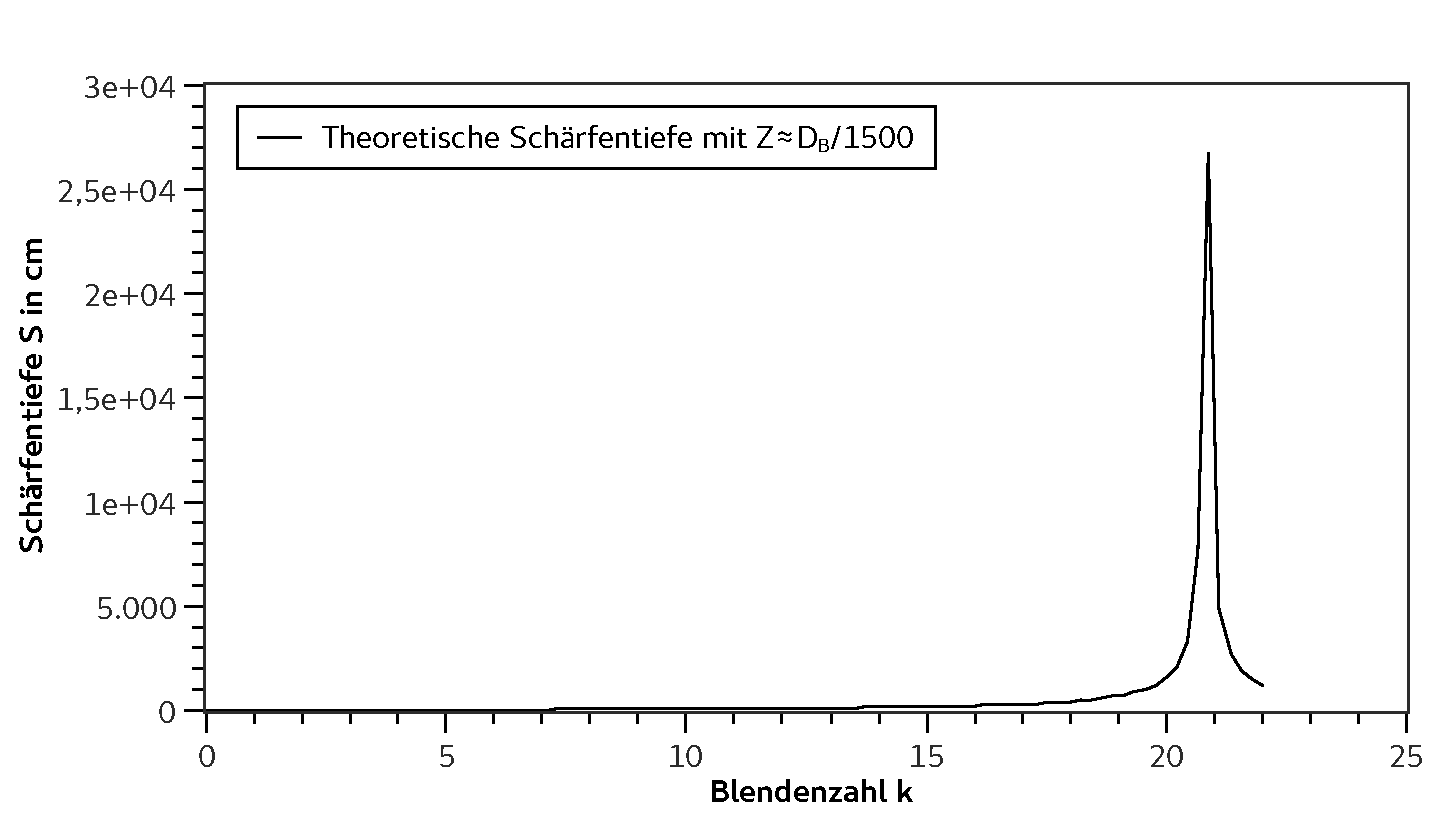
\includegraphics[width=1\textwidth]{fig_scharf_tief_theo}
		\centering
		\caption{
			Die rote Funktion ist theoretische Schärfentiefe nach \cref{eq_scharf_tief} mit entsprechenden Parametern.
			Die Schärfentiefe $S_text{theo}$ divergiert gegen hohe Werte bei $k\approx21$.
			Dies entspricht dem Fall $g\approx d_h$, sodass $d_f$ divergiert.
			}
		\label{fig_scharf_tief_theo}
		\centering
	\end{figure}

	\subsection{Diskussion}
	%TODO Bezug/Nutzen oder sonst was
	%TODO auch hier die Hypothese wiederholen
	%TODO keine Messwerte hier, nach manchen Menschen, zumindest "direkt" erstellte Diagramme net hier, auch wenn Lesbarkeit-bla
	
	%TODO Siemensstern mitte nicht gut in Mitte
	\section{Schlussfolgerung}
	%TODO Rückgriff auf Hypothese und drittes Nennen dieser
	
	%TODO Quellen zitieren, Websiten mit Zugriffsdatum
	%TODO Verweise auf das Laborbuch (sind erlaubt)
	%TODO Tabelle + Bilder mit Beschriftung
	\printbibliography
\end{document}
